\section{Recommendation systems}
\only<presentation>{
  \begin{frame}
    \tableofcontents[ 
    currentsection, 
    hideothersubsections, 
    sectionstyle=show/shaded
    ] 
  \end{frame}
}

\begin{frame}
  \begin{figure}[H]
    \centering
    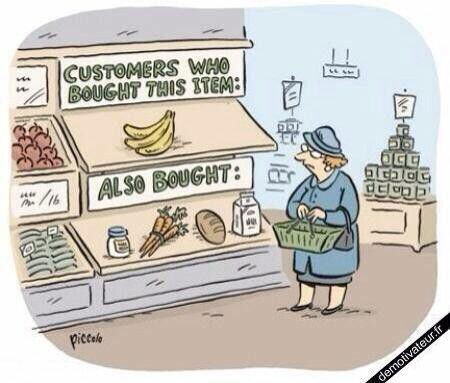
\includegraphics[width=0.4\textwidth]{../figures/recommendation}
    \only<article>{\caption{The recommendation problem}}
    \label{fig:recommendation}
  \end{figure}
  \only<article>{In many machine learning applications, we are dealing with the problem of proposing one or more alternatives to a human. The human can accept zero or more of these choices. As an example, when using an internet search engine, we typically see two things: (a) A list of webpages matching our search terms (b) A smaller list of advertisements that might be relevant to our search. At a high level, }
  \begin{block}{The recommendation problem}
    At time $t$
    \begin{enumerate}
    \item A customer $\bx_t$ appears. \only<article>{For the internet search problem, $\bx_t$ would at least involve the search term used.}
    \item We present a choice $a_t$. \only<article>{For the matching website, the choice is ranked list of websites. For the advertisements, however, it is typical }
    \item The customer chooses $y_t$. \only<article>{This might include selecting one or more of items suggested in $a_t$. The choice of the customer may not be directly visible.}
    \item We obtain a reward $\rho(a_t, y_t) \in \Reals$. \only<article>{Typically this is a payment either from the customer or an advertiser.}
    \end{enumerate}
  \end{block}
\end{frame}

\begin{frame}
  \begin{figure}[H]
    \centering
    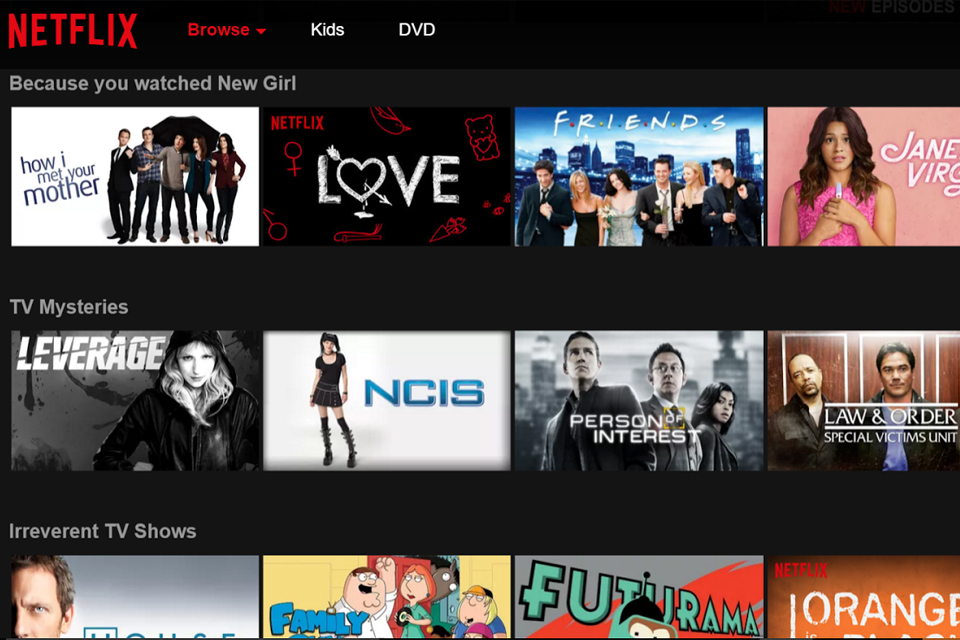
\includegraphics[width=0.9\textwidth]{../figures/netflix}
    \caption{The Netflix recommendation problem}
    \label{fig:netflix}
  \end{figure}
  \only<article>{
    \begin{example}
      In the case of Netflix and related services, we would like to suggest movies to users which they are more likely to watch, as shown in Figure~\ref{fig:netflix}. However, how can we tell which movies those can be? It is probably not useful to just recommend them to rewatch a previously watched movie. We need to somehow take into account information across our user database: if somebody watched mostly the same films as you, then maybe you'd be interested in watching those movies she has that you haven't seen.

      In the Netflix catalogue, in particular, users also post reviews of the movies they have watched, as shown in Figure~\ref{fig:user-ratings}. This allows us to be able to guess the ratings of users from previous user's ratings.
    \end{example}
  }
\end{frame}
\begin{frame}
  \begin{figure}[H]
    \centering 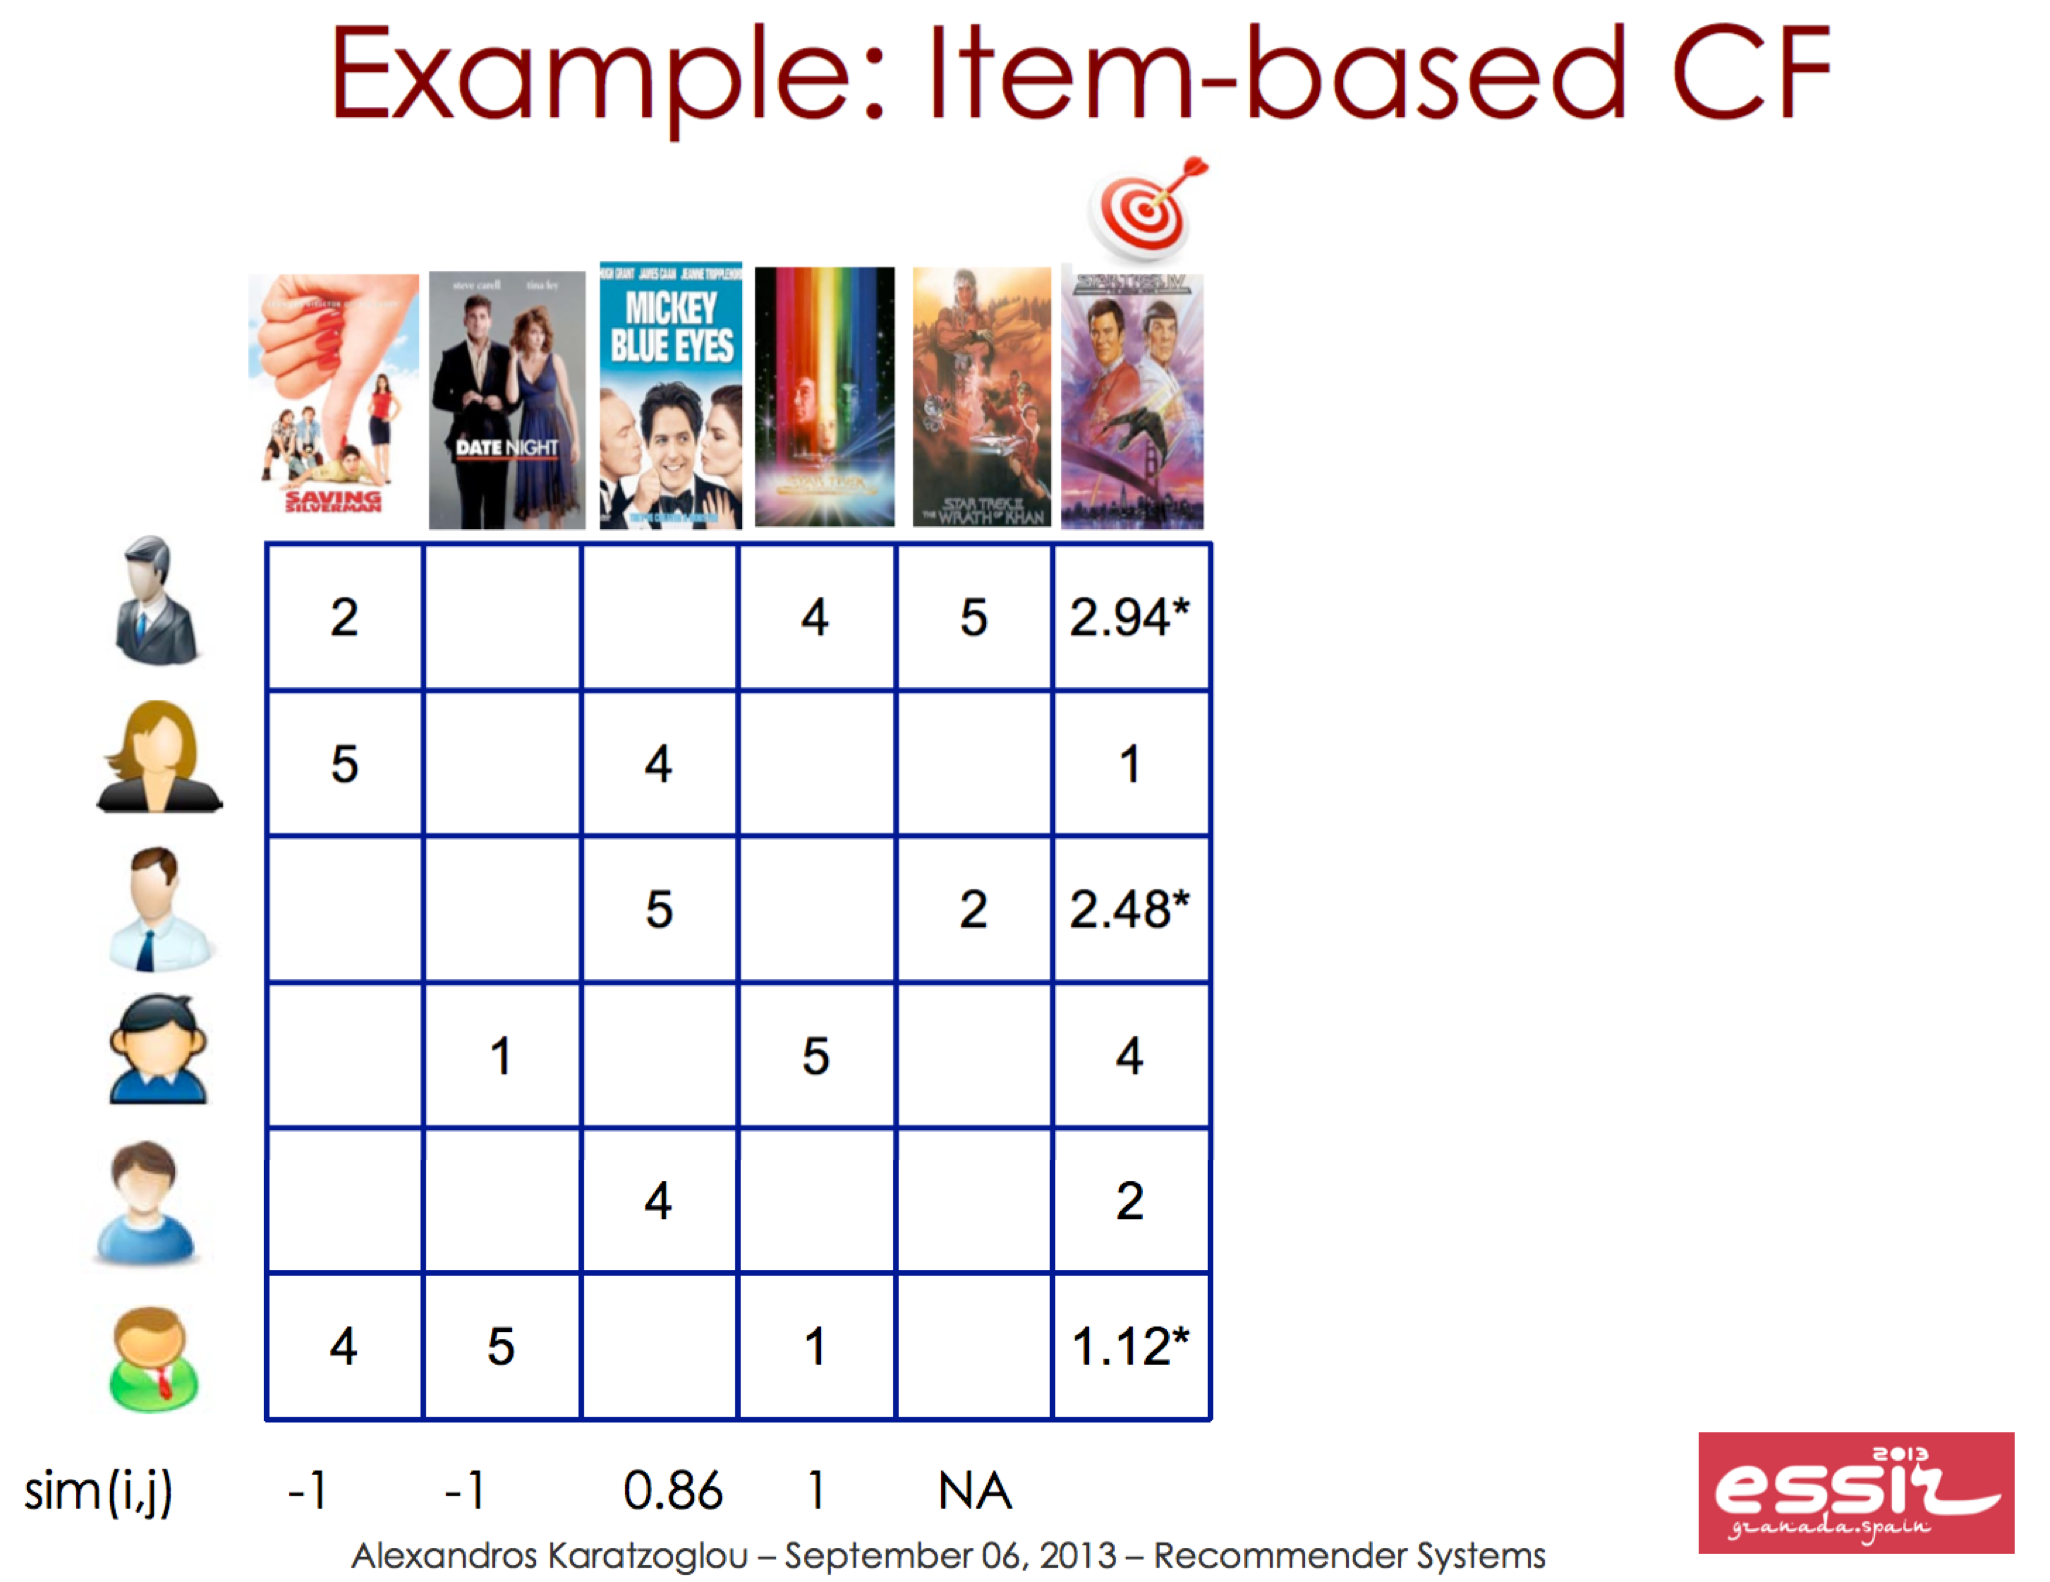
\includegraphics[width=0.9\textwidth]{../figures/recommendationExample-1}
    \caption{User ratings}
    \label{fig:user-ratings}
  \end{figure}

\end{frame}

\begin{frame}
\frametitle{Predictions based on similarity}
\begin{block}{Collaborative filtering}
  \begin{itemize}
  \item \alert{Similar users have similar tastes}. \only<article>{For example, consider two users $t, u$ who have each watched a set of movies $\CM_t$ and $\CM_u$ respectively, and $\CM_{t,u} = \CM_t \cap \CM_u$ is the set of common movies. If their ratings are the same for those movies, i.e. $x_{t.m} = x_{u,m} \forall m \in \CM_{t,u}$, then it's a good guess that they might have the same ratings for movies they have not both watched. }
  \item That means we can use similar user's \alert{ratings} to predict the ratings for other users. 
\only<article>{The advantage is that ratings are readily available. The disadvantage is that new users have too few data to be matched to other users.}
  \end{itemize}
\end{block}
\begin{block}{Content-based filtering.}
  \begin{itemize}
  \item Users typically like similar items. \only<article>{For example, a horror movie fan typically rates horror movies highly.}
  \item That means we can one user's ratings and \alert{item information} to predict their ratings for other items. \only<article>{In this scenario}
  \end{itemize}
\end{block}
\end{frame}


\begin{frame}
  \frametitle{$k$-NN for similarity}
  \begin{exercise}
    \begin{itemize}
      \item Define a distance $d : \CX^M \times \CX^M \to \Reals_+$ between user ratings.
      \item Apply a $k$-NN-like algorithm to prediction of user ratings from the dataset.
    \end{itemize}
  \end{exercise}
\end{frame}
\begin{frame}
\begin{block}{From distance to similarity}
    Let us define a similarity $w_{ij}$ between two users so that
    \[
    \sum_{j \neq i} w_{i,j} = 1.
    \]
    Then we can define the inferred ratings 
    \[
    \hat{x_{u.m}} = \sum_{j \neq i} w_{i,j} = 1.
    \]
  \end{block}

  \begin{example}[$k$-nearest neighbours]
    $w_{i,j} = 1/k$ for the $k$ nearest neighbours with respect to $d$.
  \end{example}


  \begin{example}[Weighted distance]
    \[
    w_{i,j} = \frac{\exp[-d(i,j)]}{\sum_{k \neq i} \exp[-d(i,j)]}
    \]
  \end{example}
\end{frame}

\begin{frame}
  \begin{block}{A naive distance metric}
    \[
    d(i,j) = \|\bx_i - \bx_j\|
    \]
  \end{block}
\end{frame}

\begin{frame}
  \frametitle{Preferences as clusters}
  \only<article>{As a simple model, we can assume that each person belongs to a \alert{type}. Every type has the same preferences over films. In the simplest possible model, a user of type $c_i$ that has watched a movie $m$ will rate the film deterministically $x_{c,m}$. More generally, we can assume the following model.}
  \begin{figure}[H]
    \centering
    \begin{tikzpicture}
      \node[RV] at (2,0) (data) {$\bx_t$};
      \node[RV,hidden] at (0,0) (cluster) {$c_{t}$};
      \draw[->] (cluster)--(data);
      \uncover<2>{
        \node[RV,hidden] at (0,1) (param) {$\param$};
        \draw[->] (param)--(cluster);
        \draw[->] (param)--(data);
      }
    \end{tikzpicture}
    \caption{Preference model}
    \label{fig:preference-model}
  \end{figure}
  \begin{block}{Preference model}
    \begin{itemize}
    \item User $t$.
    \item User type $c_t \in \CC$. \only<article>{For simplicity, we can think of there being a finite number of types $\CC = \{1, \ldots, n\}$.}
    \item User ratings  $\bx_t$ with $x_{t,m} \in \CX$ rating for movie $m$. \only<article>{As an example, $\CX = \{0, 1, 2, 3, 4, 5\}$, with $0$ meaning no rating given. This is important, since }
    \item Preference distribution $P_\param(\bx_{t} = \bx | c_t = c)$.\only<article>{Typically, we can assume that ratings are independent given the type
        \[
        P_\param(\bx_{t} = \bx | c_t = c) = \prod_{m=1}^M P_\param(x_{t,m} = x_m | c_t = c),
        \]
        so that a single (vector) parameter $\param_{c,m}$ will describe the distribution of ratings for a particular movie $m$ and type $c$, i.e.  $P_\param(x_{t,m} = x_m | c_t = c) = P_\param(x_{t,m} = x_m | c_t = c)$.}
    \end{itemize}
  \end{block}
\end{frame}
%%% Local Variables:
%%% mode: latex
%%% TeX-engine: xetex
%%% TeX-master: "notes.tex"
%%% End:
